\chapter{Einführung}
Am 25. Oktober 2018 wurde bei Christies das erste Gemälde verkauft, welches durch künstliche Intelligenz erschaffen
wurde \cite{Christies:PortraitEdmundBelamy}. Auf etwa 10'000 USD geschätzt, brachte es dem Anbieter doch über
432'500 USD ein. Es zeigt das Porträt einer fiktiven  Person namens Edmond Belamy,
trainiert mit über 15'000 Bildnissen verschiedener Epochen \cite{nzz:1:belamy}. Ob dieses \glqq Gemälde\grqq{} nun
als kreatives Werk angesehen werden kann, ist sehr umstritten und wird auch nicht weiter behandelt.
Es steht viel mehr der Künstler im Mittelpunkt. Der Künstler namens \Gls{GAN}.
\para
Doch wieso ist so ein \Gls{GAN} überhaupt von Interesse? Leser mit Vorkentnissen im Bereich der künstlichen neuronalen
Netzwerke haben wahrscheinlich schon gemerkt, dass es nicht trivial ist, neue Daten aufgrund von Bestehenden zu generieren.
Für alle, welche nicht Wissen, was gemeint ist, sei gesagt, dass ein \Gls{KNN} Daten klassifizieren kann, aber nicht unbedingt
neue Daten erzeugen. Das Generieren erfordert weitaus mehr.
Es soll ein kleines Beispiel behandelt werden, um aufzuzeigen, was gemeint ist. Die Idee zu diesem Gedankenexperiment
stammt von \glqq Computerphile\grqq{} \cite{youtube:gan}.
Ein neuronales Netz lernt auf Basis von Input-Daten ein Modell. In diesem Fall gibt es deren drei Input-Daten, welche in der Abbildung 1.1
dargestellt werden. Wie erkannt werden kann, sind diese Datenpunkte sehr zufällig gewählt.
\begin{figure}[h!]
    \begin{center}
        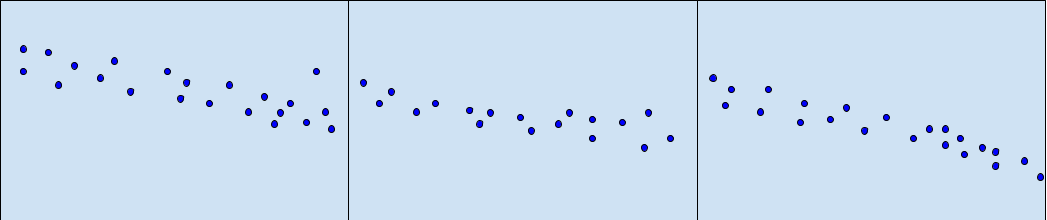
\includegraphics[width=0.6\textwidth]{../common/02_main/resources/00_input.png}
    \end{center}
    \caption{Input-Daten für \Gls{KNN}}
    \label{fig:Input-Daten für KNN}
\end{figure}
\newpage
Das Modell, welches das \Gls{KNN} lernt, kann wie in Abbildung 1.2 ersichtlich visualisiert werden. Es bildet eine möglichst
gute Annäherung an alle Datenpunkte ab.
\begin{figure}[h!]
    \begin{center}
        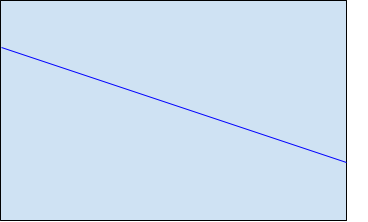
\includegraphics[width=0.4\textwidth]{../common/02_main/resources/01_modell.png}
    \end{center}
    \caption{Gelerntes Modell}
    \label{fig:Gelerntes Modell}
\end{figure}
Doch wie kann nun ein neues Sample, welches möglichst mit den Input-Daten korreliert, erzeugt werden? Das einzige, was
das Netzwerk wahrscheinlich kann, sind zufällige Datenpunkte auf der Modellgeraden bestimmen.
\begin{figure}[h!]
    \begin{center}
        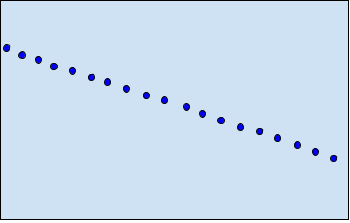
\includegraphics[width=0.4\textwidth]{../common/02_main/resources/02_generierte_punkte.png}
    \end{center}
    \caption{Generiertes Sample aufgrund von gelerntem Modell}
    \label{fig:Generiertes Sample aufgrund von gelerntem Modell}
\end{figure}
In der Abbildung 1.3 kann entnommen werden, dass dies nicht wirklich natürlich wirkt und nicht mit den Input-Daten übereinstimmt.
Die Frage stellt sich nun, wie also solche natürlich wirkenden Samples erzeugt werden können? Eine Antwort darauf liefert
\Gls{GAN}. Die vorliegende Arbeit geht der Fragestellung nach, wie diese \glqq Generative Adversarial Networks\grqq{}
funktionieren.